\chapter{METODOLOGIA}\label{chap:metodologia}

Este trabalho possui pesquisa aplicada\ldots

Utilizamos programação em linguagem C para sistema Linux, com metologia de desenvolvimento em código aberto.

Utilizamos, inicialmente, um sensor inercial modelo MPU-6050 anexado a uma Raspberry Pi 3B, conforme exibido na figura abaixo:~\ref{fig:figura22}.

\begin{figure}[H]
    \centering
    \caption{Sensor MPU-6050 anexado à Raspberry Pi}\label{fig:figura22}
    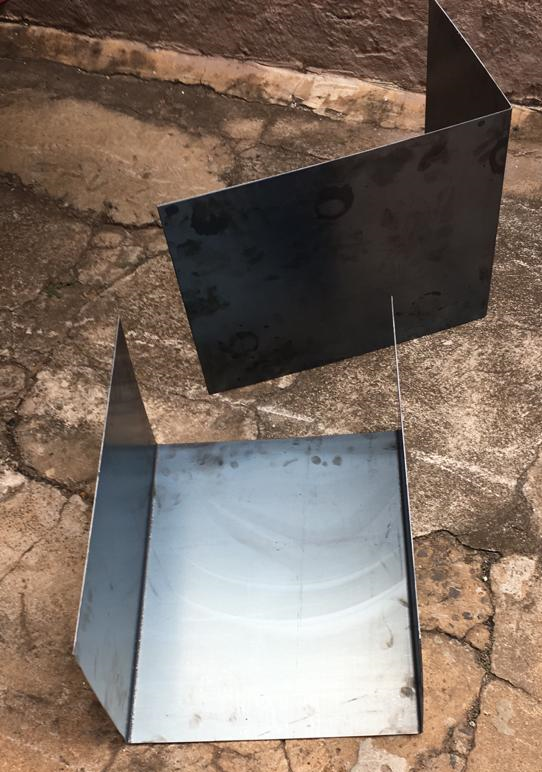
\includegraphics[width=0.7\textwidth]{figuras/figu22.png}
    \fonte{Autores}
\end{figure}
